\documentclass[11pt,a4paper]{article}
\usepackage[utf8]{inputenc}
\usepackage{textcomp}
%\usepackage{amsmath}
%\usepackage{amsfonts}
%\usepackage{amssymb}
\usepackage{fancyhdr}
%\usepackage{graphicx}
\usepackage{CJK}
\usepackage{listings}
%\usepackage{url}
%\usepackage[unboxed,small]{cwpuzzle}
\usepackage[left=2cm,right=2cm,top=3cm,bottom=2.5cm]{geometry}
%\usepackage[inline]{enumitem}
%\setitemize{listparindent=\parindent}
\usepackage{indentfirst}
\usepackage{graphicx}
\usepackage[labelformat=empty]{caption}

\parskip=4pt

%\pagestyle{fancy}
%\lhead{}
%\rhead{}

\begin{document}
\DeclareGraphicsExtensions{.pdf,.png,.jpg}

\begin{center}
\textbf{\Large Artificial Intelligence Final Project Report}\\[1em]
\begin{CJK}{UTF8}{bsmi}
{\Large Group 29 SmartShell}\\[1em]
{\large b99902054 資工四 薛祐婷, }
{\large b99902108 資工四 李昀儒 }\\[1em]
{\large r03922093 資工碩一 王友伶, }
{\large r03944012 網媒碩一 陳彥儒 }\\[1em]
\end{CJK}
\end{center}
\section*{Introduction}
While working with Bash, it is tedious for most of the users to type repeated commands. 
Even with the Bash build-in auto-completion feature, sufficient characters must be provided to solve ambiguity of prefix.
If the commands can be auto-completed with just a few number of characters typed, it saves a lot of time. 
Although around 72\%, according to the past research [1], of the commands can be predicted from history file, 
it still work especially when users are coding or doing another work which will type repeated commands in a period. 
The common solution for this condition is reverse search, 
which only find the latest commands of whose prefix corresponds to what the user just type. 
However, it still left something to be desired. 
Therefore, we introduce a better shell which can preform customized auto-completion with information extracted from user history instead of just finding the latest one.

\section*{Problem definition}
What we want to do is to introduce a "smarter" auto-completion shell based on command history.
Our goal is to predict the most probable command that the user want to type next. 
We compare our result with that of Bash built-in tab completion and reverse search. 
The following is the PEAS of SmartShell custom auto-completion.

\begin{itemize}
\item {\bf Performance Measure}: accuracy of the prediciton list, the speed of prediction
\item {\bf Environment}: the user and the shell
\item {\bf Actuators}: screen (stdout)
\item {\bf Sensors}: keyboard (stdin)
\end{itemize}

Besides, since our implementation is a improved shell, we regard usability as an important metric.
Our ultimate goal is to work with shell easily.

\section*{Proposed methods}
We proposed a probabilistic model to perform command prediction.
The flow of our method is as follow.
\par
The training data is from user history file. 
We maintain a window of N commands, in practice N = 500. 
In the window we compute probabilities for each commands right after another commands. 
For examples, if the training data is "ABCBCD", it implies that C probably appears right after B.
So if the previous command is B, we can predict that the next one is C.
We set the window size because the older history has less effect on the current work. 
We compute probabilities with how many times it appears.
When a new command is entered, the window moves and we dynamically update the counts. The oldest command leaves with its count decremented, and the newest command entered with its count incremented.
In the example "ABCBCD", the probability "C right after B" is 2/2 = 100\%, 
"B right after A" and "B right after C" are both 1/2 = 50\%. 
We maintain seperated set of counts for "command only" and "command with arguments".
Not only right previous one, we take previous 3 commands with different coefficient representing different weight to improve our result.
In the boundary case, the coefficient set to 0 can avoid another commands' effects. 
The system generates a command candidate list by prefix-match of the user input and all the commands ever entered by user.
The candidate list is sorted by the conditional probability described above.
One point we do better than reverse search is that we can predict without any input base on previous commands. 
Once the users want to type another different with our prediction, then we change our result from the input prefix.
Unless what users want to type cannot be found in the history file, 
our system can predict correct command with sufficient prefix.
The window then moves as new commands add to the history and compute another probability table for another auto-completion.
\par
According to research before[1], we adopt this probability model due to the high accuracy. 
It says that more previous commands leads less accuracy, which are 47.4\% and 36.9\%. 
However, we think another previous commands may help to predict. 
Therefore, we take it's opinion and fix it. 
We take some previous commands and set different coefficient to them. 
In the worst case, the accuracy will be 47.4\%, while previous one owns all weight. 
It guarantees at least accuracy and can be further improved. 
That paper is mentioned that it takes some factors such as times in one day or one week, 
we think user may work in different time, but follow his/her own habits.
That's why we compute probabilities from users' history file. 
We hope our auto-completion can maintain high accuracy for every different user. 
In computation, to make our bash realtime, we adopt a simple way that just compute how many times commands follow another. 



\section*{Implementation}
To let bash apply our custom completion predict list, 
we implement our completion function for bash, by api of the GNU Readline Library. 
GNU Readline Library provides api of reading a line from input (just like shell prompt).
We can bind keys for different functions like deleting a word, 
moving cursor to the head of the line or getting some possible command 
based on the partial command text in current line prompt. 
Furthermore, this library provided some mechanism to let user implement custom functions 
and bind the key to specific function that the user wants. 
By the library, we implement our completion function, 
where the list of the possible command completion is from our HistoryWindow class, 
which learns from the bash command history and uses the partial command text 
to predict and then generate the possible list.
\par
The figure below illustrate the flow of our program.
In the left side of this figure, there are arrows with keys, 
which are the binded with the functions we implement. 
Ctrl-n and ctrl-p not are to change the current completion command to the next/previous result.
Then, the completion our implemented are all with arguments, so we implement the new functionality of delete
all the line except the "command", which is Ctrl-k.
Since we simply use system() to execute the command, 
we have to process the path of working directory changes on our own.
That's what the right side of this figure presents.
\\
\begin{center}
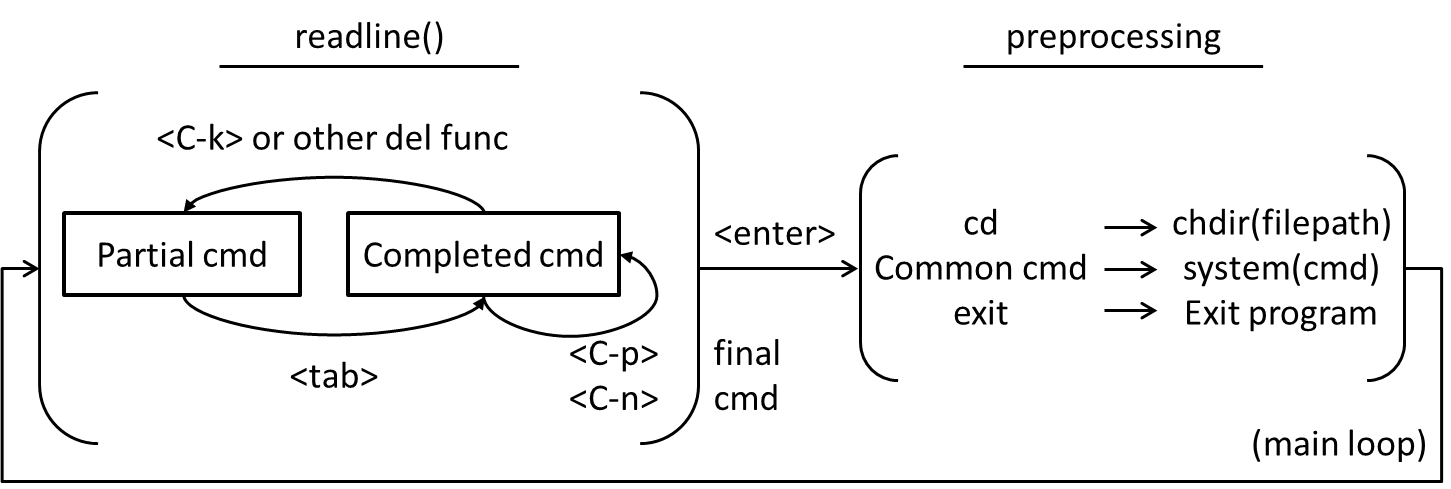
\includegraphics[scale=0.6]{pic.png}
\end{center}
\section*{Result}
To evaluate the prediction list from our model, we use a history file with about 1500~2000 commands, 
choose 500 commands as training data, fill the partial text of the next command,
and then perform our probabilistic model and reverse search to get 2 prediction commands.

We compare with 3 results of the 2 commands.
One is the accuracy of our model performing on no input partial command text, 
another is the accuracy of our model performing on half partial command text,
and the other is the accuracy of performing reverse search on half partial command text.

%result table

\begin{table}[h]
\centering
\caption{My caption}
\label{my-label}
\begin{tabular}{l|lll}
                         & \begin{tabular}[c]{@{}l@{}}Prob. model\\ (with no input)\end{tabular} & \begin{tabular}[c]{@{}l@{}}Prob. model\\ (with half cmd input)\end{tabular} & \begin{tabular}[c]{@{}l@{}}Reverse search\\ (with half cmd input)\end{tabular} \\ \hline
orina\_nlp\_history      & 0.503055                                                              & 0.543061                                                                    & 0.529543                                                                       \\
lilian\_desktop\_history & 0.444706                                                              & 0.483721                                                                    & 0.442353                                                                       \\
lilian\_lab\_history     & 0.483529                                                              & 0.517015                                                                    & 0.497647                                                                      
\end{tabular}
\end{table}


\section*{Results references}
After experiments, we find that our method gets almost the same or worse performance than reverse search. 
Because when our method cannot find any possible prediction, it output nothing.
On the other hand, reverse search can always find a prediction.
So we combine our method and reverse search only when our method cannot find any probability greater than 0,
we adopt reverse search as our method. 
To our surprise, it gets better performance than both methods, especially only take command into account. 
In the research before[1], it also suggests combination leads to better result. 
Due to different user habits for everyone, 
combination of methods can find the best prediction which is corresponding to user's habit with less bias.

\section*{Future work}

The model now use static configuration with fixed windows size.
For different user has different command typing pattern, 
the result can be improved when applying dynamic configuration.

\section*{Job responsibility of members}

\begin{CJK}{UTF8}{bsmi}
\begin{itemize}
\item 薛祐婷 - model design, model implementation, main program implementation
\item 李昀儒 - model design, model implementation, main program implementation
\item 王友伶 - model design, GNU readline library survey, main program implementaion
\item 陳彥儒 - model design, model implementation, papers about shell completion survey
\end{itemize}
\end{CJK}

\section*{Collaboration/communication mechanism}
Each member has complete freedom of deciding the time of finishing the task assigned.
We basically discuss about our project in Facebook message, 
and the one who has time will take the tasks of that time to do.
We had some meetings in CSIE Building before the due date of milestones. 
Whenever someone finish one functionality, 
the others will run the program and check whether there are bugs in short time.
Besides, we devided the task clearly in the first, 
so that we had less conflict when merging code.

\section*{References}
\begin{enumerate}
\item http://papersdb.cs.ualberta.ca/~papersdb/uploaded\_files/712/paper\_korvemaker00predicting.pdf
\item http://www.eecs.harvard.edu/hube/publications/durant-predict.pdf
\end{enumerate}

\section*{Source Code}
http://github.com/orina1123/smartshell

%\begin{enumerate}

%\lstset{
%basicstyle=\ttfamily,
%columns=flexible,
%keepspaces=true,
%upquote=true
%}
%\begin{lstlisting}
%\end{lstlisting}


%\end{enumerate}
\end{document}
